% !TEX spellcheck = en_US
% Theta min static calculations
%=================================================================================
The optimization of the minimum pitch angle is a simple adjustment which leads to a small increase in the AEP. 
The optimization was done with a brute force approach and the steady states calculations (Section \ref{steady states}). 
In control region 2 the WT should work at optimum $Cp$ and $\lambda$. 
The use of minimum pitch angle can lead to an more efficient state of the turbine at the start of region 2 and therefor increase the AEP. 
For different pitch angles the steady states where calculated. 
As optimum, min. pitch angle the angle which leads to the highest $Cp$ was chosen. 
As a result the min. pitch angle of \SI{0.5}{\degree} was determined and is shown in figure \ref{fig:theta min general}. 
During the calculation the pitch angle was optimized in a range of \SI{0}{\degree} to \SI{5}{\degree} with a step size of \SI{0.1}{\degree}.

The determined min. pitch angle of \SI{0.5}{\degree} leads to an increase in AEP of \SI{0.29}{\%} compared to min. pitch angle of \SI{0}{\degree}. 
(Calculated with Weibull parameters of TC III and $k=2$.)

\begin{figure}[tbh]
	\centering	
	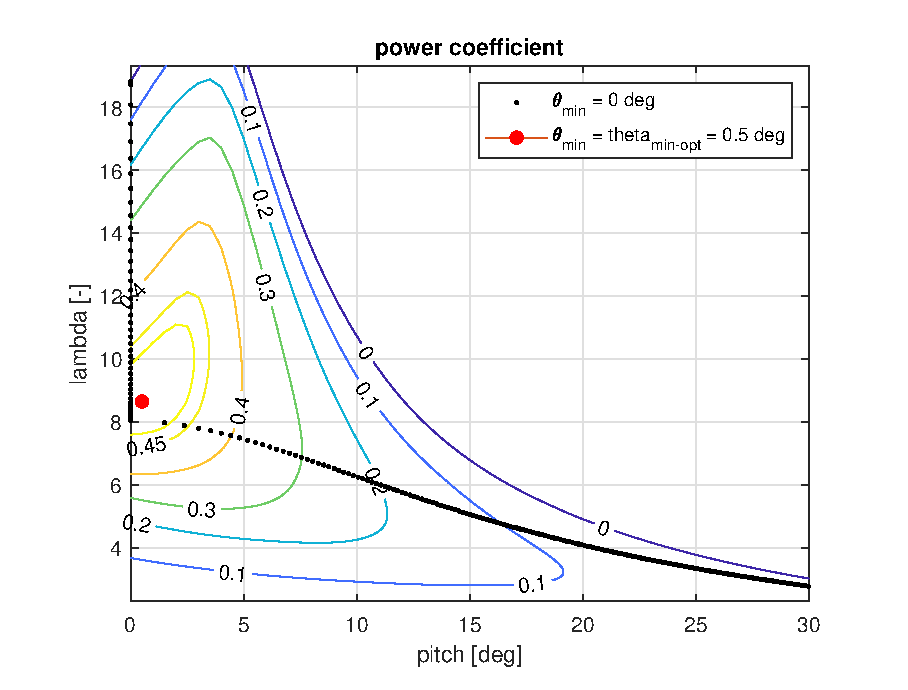
\includegraphics[width=12cm]{Figures/ThetaMinOpt}
	\caption{brute force optimization for minimum pitch angle $\theta$}
	\label{fig:theta min general}
\end{figure}